
Magic is self-replicating desire.  When we desire a thing and that thing comes to pass, that is a form of replication from our minds into either the physical world or into the minds of others.  This is the true purpose of Geometron: to create sets of self-replicating symbols in the most general sense discussed earlier in this book.  Geometron could therefore also be called Symbol Magic, as it is a system of creating symbols themselves by replicating the desire to replicate them in other human minds.

Trash Magic defines our ultimate goal in this work: the creation of the Complete Set.  A Trash Magic Complete Set is a self-replicating set which contains all the things we need as a community to live easy, comfortable lives with room for adventure in equilibrium with whatever ecosystem we are in.  This means we have technology for sanitation, clean water, illumination, heating and air conditioning, food production, production of medications and medical technology, transportation and the self-replicating media of which these documents are the seed.  And all of this technology must be built entirely from the waste we find in our immediate physical environment from the broken pieces of the old world combined with the natural flow of water, material, life, information and energy through our local ecosystem.  Only by firmly fixing in our minds this end desire and building a new system of knowledge from scratch with these ends in mind, can we break free of the existing system which forces us all to do work we hate to buy things we don't want which destroy the Earth and hurt other people. 

In order to build up this new way of seeing the world, we dive down to the deepest level of human thought, which is the subject of ``things'' in the most general sense.  What is a ``thing''? What is a collection of ``things''?  These are subjects mathematicians have tackled with vigor for a long time.  At the end of the 1800s and for the first half of the 20th century,  a collection of philosophers and mathematicians tried to build a foundation of mathematics from the theory of sets and logic.  Their goal was to build something that was ``true'' in some deep sense which turned out to be elusive.  In the views of this 20th century mathematicians created a linguistic trap in which mathematicians built increasingly meaningless worlds of symbols with no impact on the real world at all, leading to essentially an entire lost century of mathematics.  The purpose of most academic mathematics is to gain recognition required for tenure, nothing more and nothing less.

Our goals here are much more practical.  We want to build up whatever foundational ideas about language and mathematics most effectively aid us in building our new civilization from trash.  This means we want to prioritize replication at every level of definition.  In addition, we want to create our whole system based on trying to replicate the underlying desire to build up our new civilization.  To this end, we ignore the axioms of 20th century ``set theory'', and define something we call ``set magic''.  In Set Magic, we define sets to be collections of objects in the most general sense possible, just as mathematicians in the past did.  But we note that for any given set, there are a vast number of choices as to how we break that thing down into constituent elements depending on what we want to do with our definition.  In Set Magic, we always break things down into whatever collection of constituent elements are the most effective for communicating with other people what we need to communicate in order to replicate a thing.  This means we choose sets with only a few elements, each of which can be summarized with a recognizable symbol, and which are related to each other with an easy to understand relationship.  We define complex objects by building fractal structures of meaning, where things are made up of things, which are made up of things.  

In Set Magic, we can assign an icon to any thing, as well as any element which makes up a thing.  We can then use Action Geometry to make physical symbols which are easy to use to communicate meaning.  We can call these ``sigil boards'', but they can also be thought of as a generalized game board.  Geometric patterns can be drawn on cardboard with the Action Geometry sets and markers to make boards, and then we can use the clay Icon Tokens described in the Printers chapter to represent any set of objects in the most general possible sense.  Each element can then be defined as another set, and another collection of self-replicating clay tokens can be created which are used to represent that set and so on.  This can be thought of as a kind of physical symbolic hypertext, where self-replicating clay media(replicated via Geometron Printers) are arranged on self-replicating cardboard media(replicated via Action Geometry) to communicate any idea which can be parsed by the human mind to another person.  Each thing can be a link to another set and so on.  These self-replicating sets can be used to replicate anything.  They are indeed used to replicate conceptually this whole system.  

When we define sets with specific practical goals in mind, we find that the axioms of existing set theory are not satisfactory.  The axiomatic set theory which has dominated for decades(so-called ``ZFC'') has a long list of axioms which apply restrictions on what can or cannot be an element or subset that are too limiting for our purposes.  For example, we need to be able to have sets be elements of each other.  For example, I might define myself to be a set of aspects of myself, one of which is my community, but of course a community is a set of which I am an element.  While placing the set theorist inside the set they create is not strictly forbidden in old set theory, it is also not discussed.  In Set Magic we explicitly put ourselves in the sets we create.  We also put abstractions we can talk about in them, such as desires, ideas, concepts, symbolic archetypes and so on.  Again, our mathematics has as a goal communication for replication for specific goals, and we will create any symbols and ideas which further those goals.  A huge fraction of the ink spilled by set theorists has been in regards to their theory of infinite sets, which we also discard as mostly useless.  Calculus lets us squeeze infinities down into symbols which we can work with and there is not need to waste our lives trying to build structure in sets with high order infinities which do nothing to help us communicate in the real world.

Another divergence in culture from classical mathematics is that we take geometry to be more fundamental than arithmetic.  Mathematics in school is presented as the manipulation of numbers, with geometry as a secondary concern.  In our mathematics, geometric constructions are the most fundamental thing.  Geometry with meaning is a symbol, and symbols in their most general sense includes our entire technological system we are building, as well as all possible symbols to represent all possible human thoughts.  Shifting from a world view in which numbers are fundamental to one where self-replicating geometric constructions are fundamental represents a deep shift in value system. Numbers are used to determine how owns what.  They are used to buy and sell things, to track ownership, and to track people in systems of control.  The ideology of numbers has taken over society as a sort of religious cult, centered on finance, computers, and authoritarian control of bureaucrats.  When we focus our attention primarily on symbols which can replicate freely, it shifts our whole way of thinking and existing in the world.  If I want a symbol to replicate, the easier it replicates the better.  Numbers do not replicate, they are designed to help people control and dominate things in a world of consumption in which all people are in competition with one another.  Put this in the simplest possible terms, numbers help people compete and dominate and symbols help people communicate and share.  The elements of Geometron and the magic presented in this chapter represents an attempt to build a universal symbolic language which can form the basis of this new method of thought and of existence.  


The Trash Robot is a self-replicating set which we create in order to grow into the system which can ultimately create Trash Magic Complete Sets.  The Trash Robot set includes us, the people replicating the set, as part of replication is to grow the set by getting more people to join the set.  It also includes our desire to build a better world as a thing(this desire can be represented in symbols therefore it can be an element of a set).  The elements of the basic set are what are documented in this book.  As with everything here, this has a fractal structure and can be parsed multiple ways into constituent elements.  Trash Robot includes all the constructions described in this work, as well as the open brand defined by googly eyes, rainbow duct tape, things made from trash, bright colored felt on black cloth, and geometry.  Join the set, become an element!  And then help replicate the set.  If we replicate the set together and replicate the intent to build the Trash Magic Complete Set, it should be possible to build that even if it is very difficult.  From a fundamental technical standpoint, it is clear that building a Complete Set is possible, all we need is a community of people with the will to carry this out.  Building the magic set with intent is therefore enough: if it replicates and evolves, it will create what we need, even if we have no idea how to do that.



\begin{figure}
	\centering
	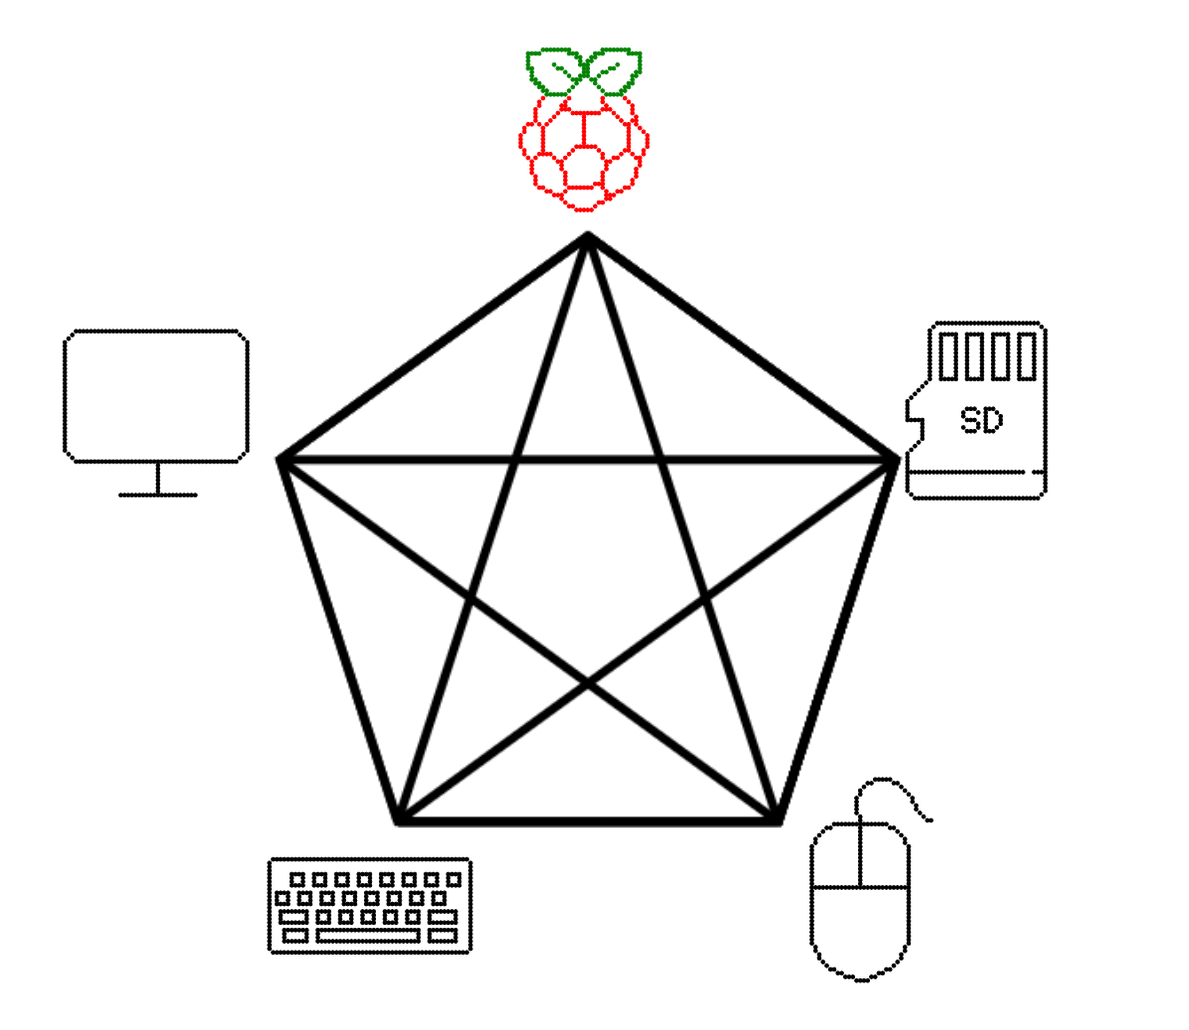
\includegraphics[width=3in]{figures/magic/pisigil.png}
	\caption[pisigil]
	{Sigil for Raspberry Pi.  This figure was created with a Geometron Map combined with symbols made with the main symbol app combined with the icon feed to make the icons.  A magician who wants to share this sigil with someone in the physical world can use these icon glyphs to print the icons in clay, replicate them and paint them to make tokens, then make a cardboard board with the symbol shown using Action Geometry.  They can then place tokens on the board to communicate about the system.  The same geometric information can be used to make self-replicating information on any Geometron server.  As above, so below: there is always a version of our geometry on the servers and one made from physical media.}
\end{figure}


\begin{figure}
	\centering
	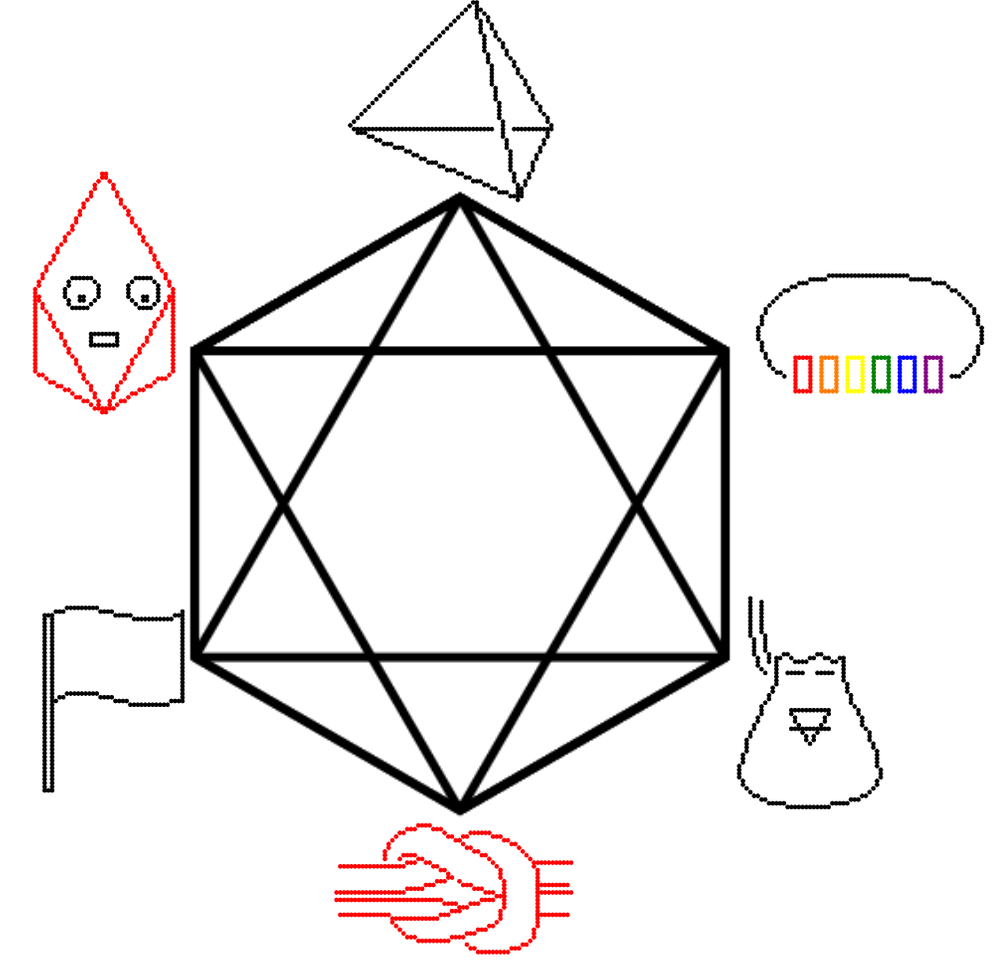
\includegraphics[width=3in]{figures/magic/actiongeometrysigil.png}
	\caption[actiongeometrysigil]
	{Sigil for Action Geometry.  Action Geometry is a self-replicating set, which is itself an element of Trash Robot, Geometron, and any other set we find it useful to put it in.  The layout of the sigil can be used to communicate relationships between things.}
\end{figure}


The symbols we use to replicate our sets are chosen purely based on what works.  Unlike the mathematical philosophers of the early 20th century, we are not seeking some higher objective ``truth''.  Our entire theory of knowledge is just based on what symbols will, if shared, replicate our intent to build Trash Magic.  Therefore we borrow from any existing symbolic framework that is convenient to use to our ends.  This can include any philosophical, religious, spiritual, mythical, cultural ideas, archetypes and symbols from anywhere.  For various reasons, this work uses the archetypes of Alchemy frequently.  The human mind finds it easy to deal with sets of five elements. And a pentagram in a pentagon connects each element to each other one.  So breaking things into five elements, and mapping them to the five elements of Earth, Air, Water, Fire and Aether can be useful.  This is not literal science! It is simply a symbolic mapping to aid in communication.  

An example of the use of alchemy dividing the code in our system up into five languages: Water(HTML), Fire(JavaScript), Air(CSS), Earth(Geometron bytecode), and Aether(PHP).  Also, the stages of creation of icon tokens are mapped to the elements with Air being the images, Aether being the glyph code for the icon, Earth being the print, Fire being the stamp, and the final colored in token being Water.  The three kinds of clay pieces are stored in black cloth bags marked with the relevant alchemy symbols.


\begin{figure}
	\centering
	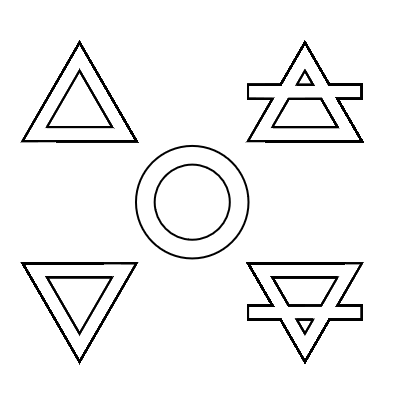
\includegraphics[width=3in]{figures/magic/alchemy.png}
	\caption[alchemy]
	{Symbols for the five elements of Alchemy.  Aether is the circle in the center.  Clockwise from upper left, the elements shown are Fire, Air, Earth, Water.  Water is blue, Air is yellow, Earth is green or brown, Aether is purple, and Fire is red.}
\end{figure}
